\documentclass[11pt]{sdm_internship}

\usepackage{graphicx}
\graphicspath{{../img/}}

\usepackage{subcaption}
\usepackage{cleveref}
\usepackage{comment}
\usepackage{wrapfig}
\usepackage{sidecap}
\pagestyle{plain}

\usepackage{hyperref}
\usepackage{url} \urlstyle{sf}
\newcommand{\email}[1]{\href{mailto:#1}{#1}}

\usepackage{xspace}

\usepackage[dvipsnames]{xcolor}
\newcommand{\addref}[1]{\colorbox{TealBlue!100}{\textcolor{white}{\textbf{$[$\ifx&#1&\ \else#1\fi$]$}}}}
\newcommand{\todo}[1]{\colorbox{Red!75}{\textcolor{white}{\textbf{TODO\ifx&#1&\else: #1\fi}}}}
\newcommand{\done}{\colorbox{YellowGreen!100}{\textcolor{white}{\textbf{DONE}}}}
\newcommand{\review}{\colorbox{YellowOrange!100}{\textcolor{white}{\textbf{REVIEW}}}}

\newcommand{\dspot}{DSpot\xspace}

\usepackage{minted}
% \usepackage{inconsolata}
% \setmonofont{Inconsolatazi4}

\usepackage{ragged2e}

\usepackage{amsthm}
\theoremstyle{definition}
\newtheorem{definition}{Definition}[section]

\title{Adapting Amplified Unit Tests for Human Comprehension}

\author{Simon \textsc{Bihel}}
\supervisorOne{Benoit \textsc{Baudry}}
\supervisorTwo{~}
\team{KTH Royal Institute of Technology}
\school{ens-Rennes}

\domain{Domain: Software Engineering --- Artificial Intelligence}

\abstract{%
  \justify{%
    \todo{}
  }
}


% Ought to be between 30 and 50 pages

\begin{document}
\maketitle

% ================================================================================
\section*{Introduction}%
\label{sec:intro}%
\addcontentsline{toc}{section}{\nameref{sec:intro}}
\todo{}


% ================================================================================
\section{Background}%
\label{sec:background}
In this section, we present the landscape this thesis fits into.
We define testing (Section~\ref{ssec:software_testing}) as well as go over its use in the industry.
In particular, to understand the needs of practitioners, we present how they assess the quality of their code (Sections~\ref{ssec:elementary_metrics} and~\ref{ssec:mutation_testing}) and what it takes for a new tool to be incorporated in their workflow (Sections~\ref{ssec:need_easy} and~\ref{ssec:cognitive_support_unit_test}).

% --------------------------------------------------------------------------------
\subsection{Software Testing}%
\label{ssec:software_testing}
In this section we give a definition for the test activities and their actors, the different abstraction levels of tests, and our precise object of study, unit tests.

\todo{Why are we testing software and how do we do it}

\todo{Say that the formal definitions aren't totally necessary}

% - - - - - - - - - - - - - - - - - - - - - - - - - - - - - - - - - - - - - - - -
\subsubsection{Test Activities}%
\label{sssec:test_activities}
\todo{}

Testing is about verifying that a system, for a certain scenario, follows a certain behaviour that was previously defined.
The \emph{System-Under-Test} (SUT), in our domain a software system, has a set of components $C$.
A scenario is sequence of stimuli that target a subset of components, and trigger both responses from the SUT and changes in the state of its components.
From~\cite{barr2015oracle}, we have the following definition for test activities:

\todo{can you add a subjective judgement here? like ``here is a well written definition''}

\begin{definition}[Test Activities]
  For the SUT $p$, $S$ is the set of stimuli that trigger or constrain $p$'s computation and $R$ is the set of observable responses to a stimulus of $p$.
  $S$ and $R$ are disjoint.
  Test activities form the set $A = S\uplusR$.
\end{definition}

\begin{wrapfigure}{r}{25em}
  \centering
  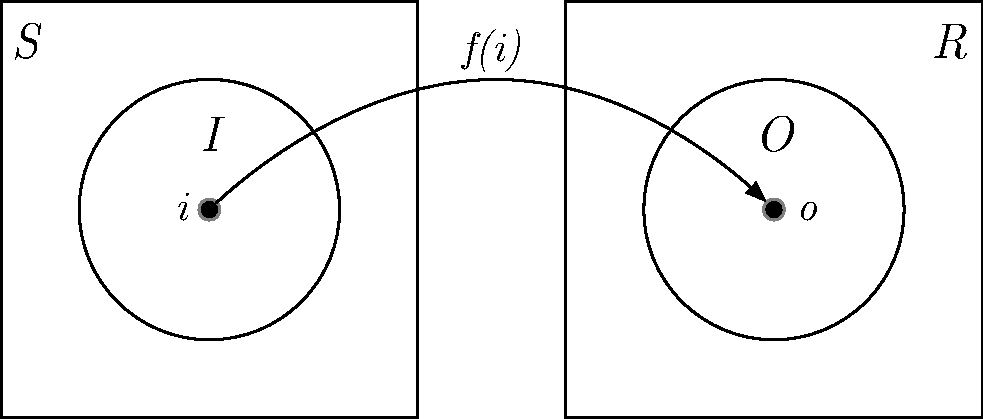
\includegraphics[width=25em]{stim_and_obs}
  \caption{Space representation of a test.}%
  \label{fig:test_activity}
\end{wrapfigure}

\figurename~\ref{fig:test_activity}

\begin{definition}[Test Oracle]
  \todo{}
\end{definition}

\begin{definition}[Regression Testing]
  \todo{}
\end{definition}

% - - - - - - - - - - - - - - - - - - - - - - - - - - - - - - - - - - - - - - - -
\subsubsection{Levels of Testing}%
\label{sssec:levels_testing}
\begin{wrapfigure}{l}{25em}
  \centering
  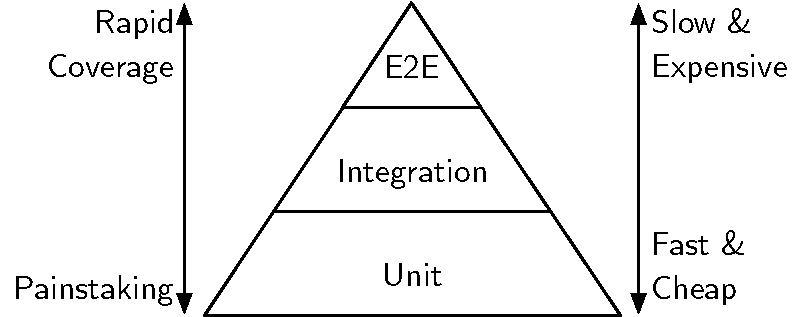
\includegraphics[width=25em]{test_pyramid}
  \caption{A view of the test pyramid.}%
  \label{fig:test_pyramid}
\end{wrapfigure}

In the case of software testing, the SUT can be different elements of a program, i.e.\ it can belong to different levels of abstraction.
One can decide to test a whole program, by manually giving inputs and verifying that the output is correct.
Or one could test individual functions, having a more control over the behaviour of each elements.

These levels of test abstraction can be visualised with a test pyramid, as shown in \figurename~\ref{fig:test_pyramid}.
Tests are generally separated into three distinct categories.
The top category is for the End-to-End tests, which means testing the program as a whole.
Whilst it allows for directly evaluating the well behaviour of the program, each test is costly in time and resources because the whole program has to be run.
Not only will each component be run, whether or not it requires testing, but time will also be spent on call to libraries that are already tested.
At the other end of the test spectrum are the unit tests.
The goal is to test each and every component of the program (e.g.\ every function), as an individual and isolated from the rest of the program.
Running a single component is faster than running the whole program, but require much more work from the person writing tests, as every component needs its set of tests.
In between the two testing practices are the integration tests, which aim at ensuring the well collaboration of components.

\todo{metaphor about rotating gears?}

\todo{how tests are automated}

% - - - - - - - - - - - - - - - - - - - - - - - - - - - - - - - - - - - - - - - -
\subsubsection{Unit Testing}%
\label{sssec:unit_testing}

\todo{not clear what a unit is\cite{runeson2006survey}}
\begin{figure}
  \centering
  \begin{minted}[linenos]{java}
testIterationOrder() {
  TreeList tl = new TreeList(10);
  for (int i = 0; i < size; i++) {
    tl.add(i);
  }
  int i = 0;
  ListIterator it = tl.listIterator();
  while (it.hasNext()) {
    Integer val = it.next();
    assertEquals(i++, val.intValue());
  }
}
  \end{minted}
  \caption{Example of a unit test.}%
\label{fig:test_example}
\end{figure}

\begin{definition}[Test Suite]
  \todo{}
\end{definition}

% --------------------------------------------------------------------------------
\subsection{Elementary Metrics}%
\label{ssec:elementary_metrics}
\todo{used to measure how thoroughly tested is a system}

\todo{What are the basic metrics}

\todo{What are their limits}

% --------------------------------------------------------------------------------
\subsection{Mutation Testing}%
\label{ssec:mutation_testing}
\begin{wrapfigure}{l}{9em}
  \centering
  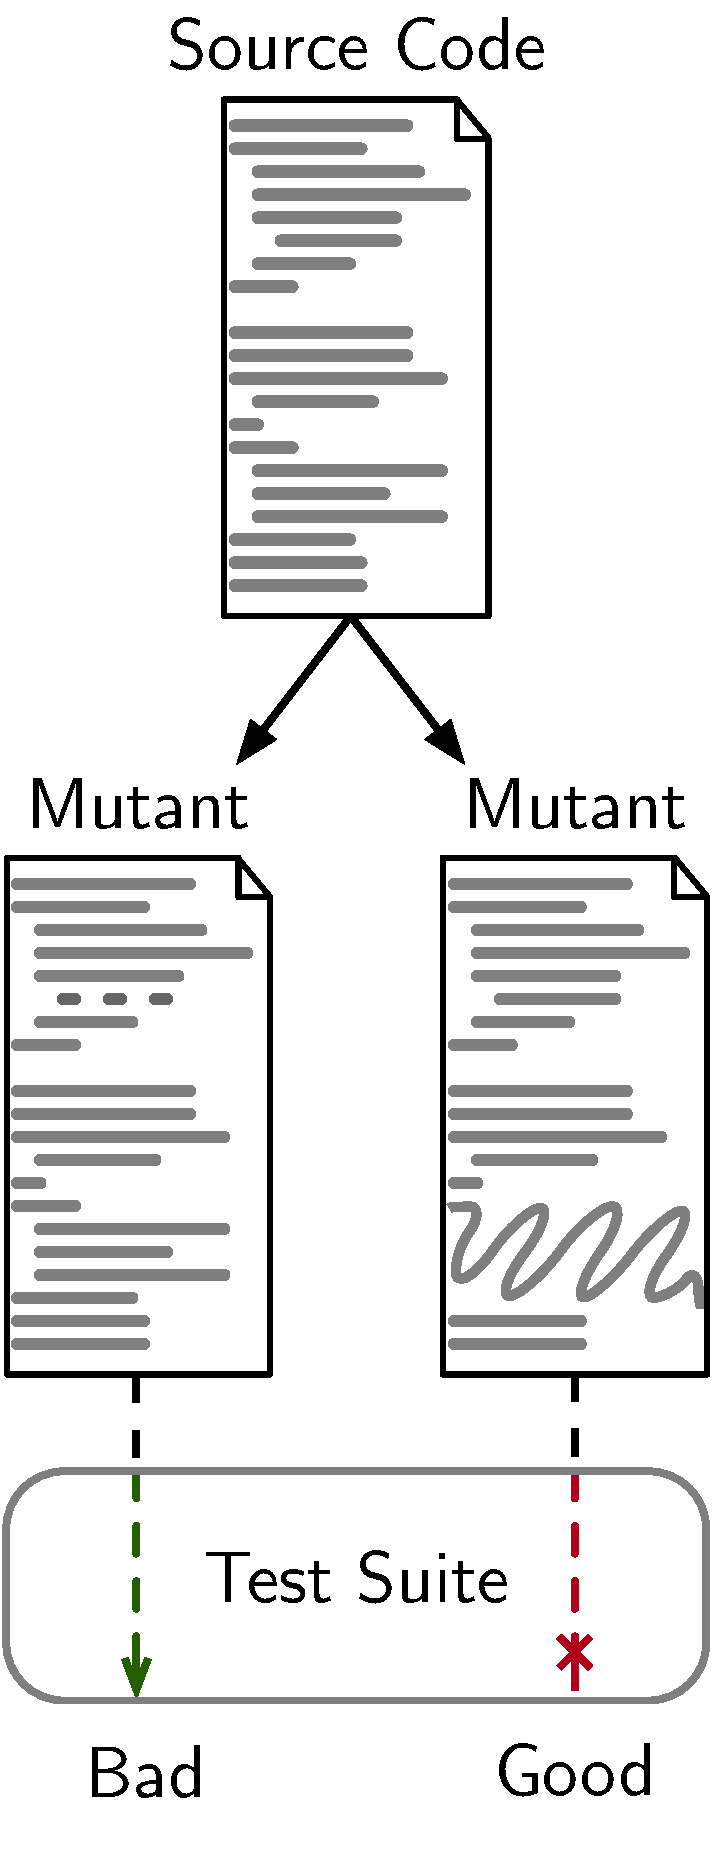
\includegraphics[width=9em]{mutation_testing_report}
  \caption{Mutation testing process.}%
\label{fig:mutation_testing}
\end{wrapfigure}
% Introduction
Mutation testing is a method used to assess the quality of a test suite, grading it with a metric called \textit{mutation score}.
The idea is to insert bugs in the software and see if these faulty versions still pass the tests or not.
We call the derived versions \textit{mutants}, hence the name mutation testing.
The global process is depicted in~\figurename~\ref{fig:spaces}.
\todo{enrich}
\addref{fundational papers}

% Mutators
\todo{examples of mutators}

% Difficulties
\todo{why is it not widespread in the industry}
\begin{itemize}
  \item slow
  \item not understood (difficult to know what the improvements to the tests should be)
  \item useless mutants
  \item equivalent mutant problem
\end{itemize}
\cite{jia2011analysis}

% Pitest
PIT\footnote{\url{http://pitest.org/}}~\cite{coles2016pit} is a mutation testing tool for Java.

\todo{what is great about it}

\todo{maybe quick comparison}

\todo{it is deterministic}

% --------------------------------------------------------------------------------
% \subsection{Software Diversification}%
% \label{ssec:software_diversification}
% \todo{}

% --------------------------------------------------------------------------------
\subsection{The Need for Easy-to-use Tools}%
\label{ssec:need_easy}
\todo{easy to understand}
\todo{useful for surveys}

% --------------------------------------------------------------------------------
\subsection{Cognitive Support Tool Development}%
\label{ssec:cognitive_support}
\todo{}


% ================================================================================
\section{Test Suite Amplification}%
\label{sec:test_suite_amplification}
In this Section, we provide more context for this thesis' contribution.
\todo{}

% --------------------------------------------------------------------------------
\subsection{Related Works}%
\label{ssec:dspot_related_works}
\todo{}

% --------------------------------------------------------------------------------
\subsection{Genetic Improvement}%
\label{ssec:genetic_improvement}
\todo{}

% --------------------------------------------------------------------------------
\subsection{\dspot{}}%
\label{ssec:dspot}
\begin{SCfigure}
  \centering
  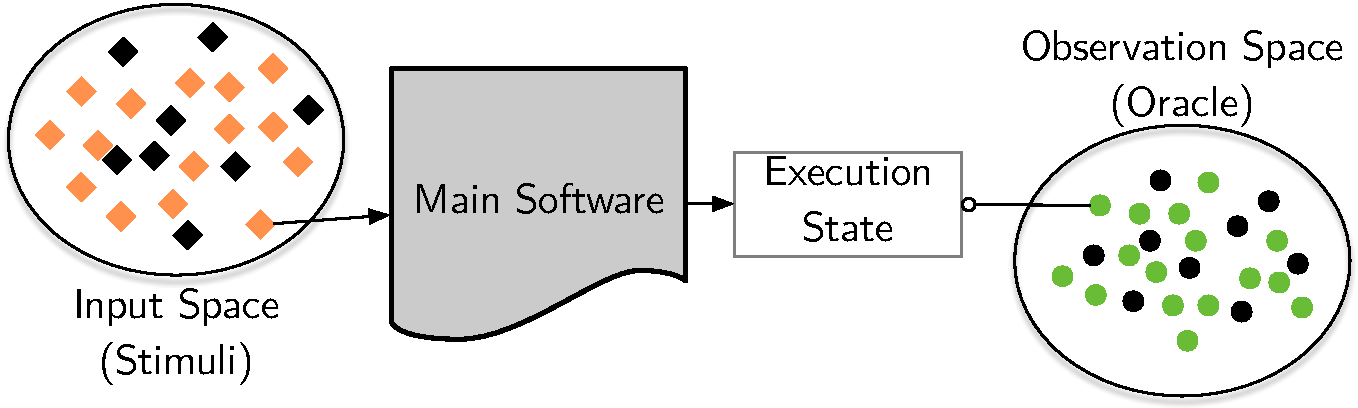
\includegraphics[width=25em]{spaces_report}
  \caption{On the left, the testing input space is composed by specified input points (orange diamonds) and unspecified input points (black diamonds). On the right, the observation space over a given program state depicts the assertions of tests. The green circles are values that are already asserted in the existing test suite, the newly added assertions are shown as black circles.}%
\label{fig:spaces}
\end{SCfigure}
\todo{}
\footnote{\url{https://github.com/STAMP-project/dspot}}\addref{dspot papers}


% ================================================================================
\section{Problem Statement}%
\label{sec:problem_statement}

% --------------------------------------------------------------------------------
\subsection{The Need for Unit Test Cases Documentation}%
\label{ssec:need_doc}
\todo{}
\cite{li2016automatically}

% --------------------------------------------------------------------------------
\subsection{The Generated Random Noise}%
\label{ssec:random_noise}
\todo{}

\todo{lack of why information}


% ================================================================================
\section{Related Works}%
\label{sec:related_works}
\todo{}

% --------------------------------------------------------------------------------
\subsection{Automatic Test Case Documentation}%
\label{ssec:test_doc}
\todo{}

% --------------------------------------------------------------------------------
\subsection{Cognitive Support for Unit Testing Review}%
\label{ssec:cognitive_support_unit_test}
\todo{}

% --------------------------------------------------------------------------------
\subsection{Source Code Change Documentation}%
\label{ssec:commit_generation}
\todo{}


% ================================================================================
\section{Contribution}%
\label{sec:contribution}
\todo{}

% --------------------------------------------------------------------------------
\subsection{Identifying Amplifications}%
\label{ssec:retrieve_amplifications}
\todo{}

% --------------------------------------------------------------------------------
\subsection{Minimisation}%
\label{ssec:minimisation}
\todo{}
\todo{put slicing before?}

% --------------------------------------------------------------------------------
\subsection{Replace or Keep}%
\label{ssec:replace_keep}
\todo{}

% --------------------------------------------------------------------------------
\subsection{Focus}%
\label{ssec:focus}
\todo{}

% --------------------------------------------------------------------------------
\subsection{Slicing}%
\label{ssec:slicing}
\todo{}

% --------------------------------------------------------------------------------
\subsection{Natural Language Description}%
\label{ssec:nl_description}
\todo{}

\todo{Focus on mutation testing}

\todo{avoid talking about mutants}
\todo{How to describe a mutant}

% --------------------------------------------------------------------------------
\subsection{Ranking}%
\label{ssec:ranking}
\todo{}


% ================================================================================
\section{Evaluation}%
\label{sec:eval}
\todo{}

% --------------------------------------------------------------------------------
\subsection{Threat to Validity}%
\label{ssec:threat_to_validity}
\todo{}

\todo{DSpot is not yet established and recognized in the community. It's is difficult to have input data (valid amplified tests)}


% ================================================================================
\section*{Conclusion}%
\label{sec:conclu}%
\addcontentsline{toc}{section}{\nameref{sec:conclu}}
\todo{}


% ================================================================================
\section*{Acknowledgments}%
\label{sec:ack}%
\addcontentsline{toc}{section}{\nameref{sec:ack}}
Thanks to Benoit Baudry and Martin Monperrus for their guidance.
Thanks to Benjamin Danglot for his collaboration and all his work on \dspot.
Thanks to Zimin Chen, Nicolas Harrand, He Ye and Long Zhang for making daily life enjoyable.
This internship was supported by the Fondation Rennes 1 and its patrons.
Many thanks to KTH for hosting me.


% ================================================================================
\bibliographystyle{ieeetr}%
\bibliography{../bibl}
\addcontentsline{toc}{section}{References}

\end{document}
